\section{ATIVIDADES REALIZADAS E RESULTADOS OBTIDOS}
\label{sec:ativ_real}
\par{Neste período de estudos, foi desenvolvido e implementado um Classificador Sismológico avançado, empregando redes neurais convolucionais para a classificação de espectrogramas de eventos sismológicos. Este algoritmo foi concebido para distinguir entre eventos naturais e antropogênicos, proporcionando uma ferramenta robusta para análises sismológicas detalhadas.}

\par{O Classificador Sismológico foi desenvolvido em Python e é mantido em um repositório no GitLab, sob a colaboração entre o Laboratório de Planetologia e Geociências da Universidade de Nantes, França, e o setor de Sismologia do IPT. O código desenvolvido permite desde a aquisição até a análise das métricas de desempenho do modelo.}

\subsection{Desenvolvimento e configuração do sistema}
\label{subsec:desenvolvimento}
\par{O sistema foi estruturado para operar de maneira dinâmica e eficiente, permitindo a aplicação do algoritmo de classificação francês de forma integrada com os procedimentos de aquisição de dados sismológicos. A instalação e configuração do ambiente para o classificador foram automatizadas por meio de scripts, facilitando a reprodução e a execução em diferentes infraestruturas computacionais.}

\par{Para a coleta de dados, foi estabelecida uma pipeline que integra o download, a filtragem e o armazenamento dos dados sismológicos, utilizando catálogos do MOHO (IAG-USP) para garantir a obtenção de eventos naturais. A classificação dos eventos foi realizada considerando distintos períodos do dia para discernir entre eventos naturais e antrópicos, com uma análise adicional da forma de onda no software Snuffler.}

\subsection{Testes e validação do Classificador}
\label{subsec:testes_validacao}
\par{O classificador foi testado utilizando um conjunto de dados rigorosamente selecionado, composto por eventos rotulados como naturais por especialistas. Esta fase de testes foi crucial para validar a precisão do classificador na discriminação entre eventos antrópicos e naturais, ajustando parâmetros e refinando o modelo conforme necessário.}

\par{Os resultados dos testes foram encorajadores, mostrando uma boa capacidade do modelo em identificar corretamente a natureza dos eventos sismológicos. As métricas de desempenho, como precisão e recall, foram calculadas e apresentaram resultados satisfatórios, reforçando a eficácia do classificador desenvolvido.}

\par{Adicionalmente, foram realizados ajustes baseados nos resultados dos testes, incluindo a otimização da captura de dados e do pré-processamento, para melhorar a acurácia das classificações.}

\subsection{Implicações e futuras diretrizes}
\label{subsec:implicacoes}
\par{Os avanços alcançados com o desenvolvimento deste classificador sismológico abrem novas perspectivas para a análise de dados sismológicos no Brasil. Com a capacidade de discriminar de forma eficiente entre eventos naturais e antropogênicos, o classificador é uma ferramenta valiosa para o monitoramento ambiental e para a pesquisa geológica.}

\par{Recomenda-se a continuidade do desenvolvimento do sistema, com atualizações regulares do modelo e a integração de novas técnicas de análise de dados sismológicos. Além disso, é crucial manter a colaboração entre instituições de pesquisa nacionais e internacionais para aprimorar constantemente as capacidades de monitoramento sismológico do país.}

\par{A implementação do classificador em outras regiões e para diferentes tipos de dados sismológicos também será explorada, visando expandir sua aplicabilidade e contribuir para um conhecimento mais profundo da dinâmica sismológica regional e global.}

\subsection{Análise de Eventos em Horários Não Comerciais}
\label{subsec:nao_comerciais}


\begin{figure}[ht!]
	\captionsetup{justification=justified, singlelinecheck=false, width=1\textwidth}
    \caption{Mapa do Brasil mostrando pontos de interesse e os epicentros dos eventos classificados como detonações e sismos. Foram detectados um total de sessenta e sete (67) eventos associados a detonações no período, classificados a partir do horário de ocorrência e da forma de onda, além do plano de fogo fornecido, com magnitudes mínima e máxima de 0.4 e 3.0 MLv, respectivamente.}
    \begin{mdframed}[
        linecolor=black,
        linewidth=1pt,
        roundcorner=10pt,
    ]
    \begin{center}
    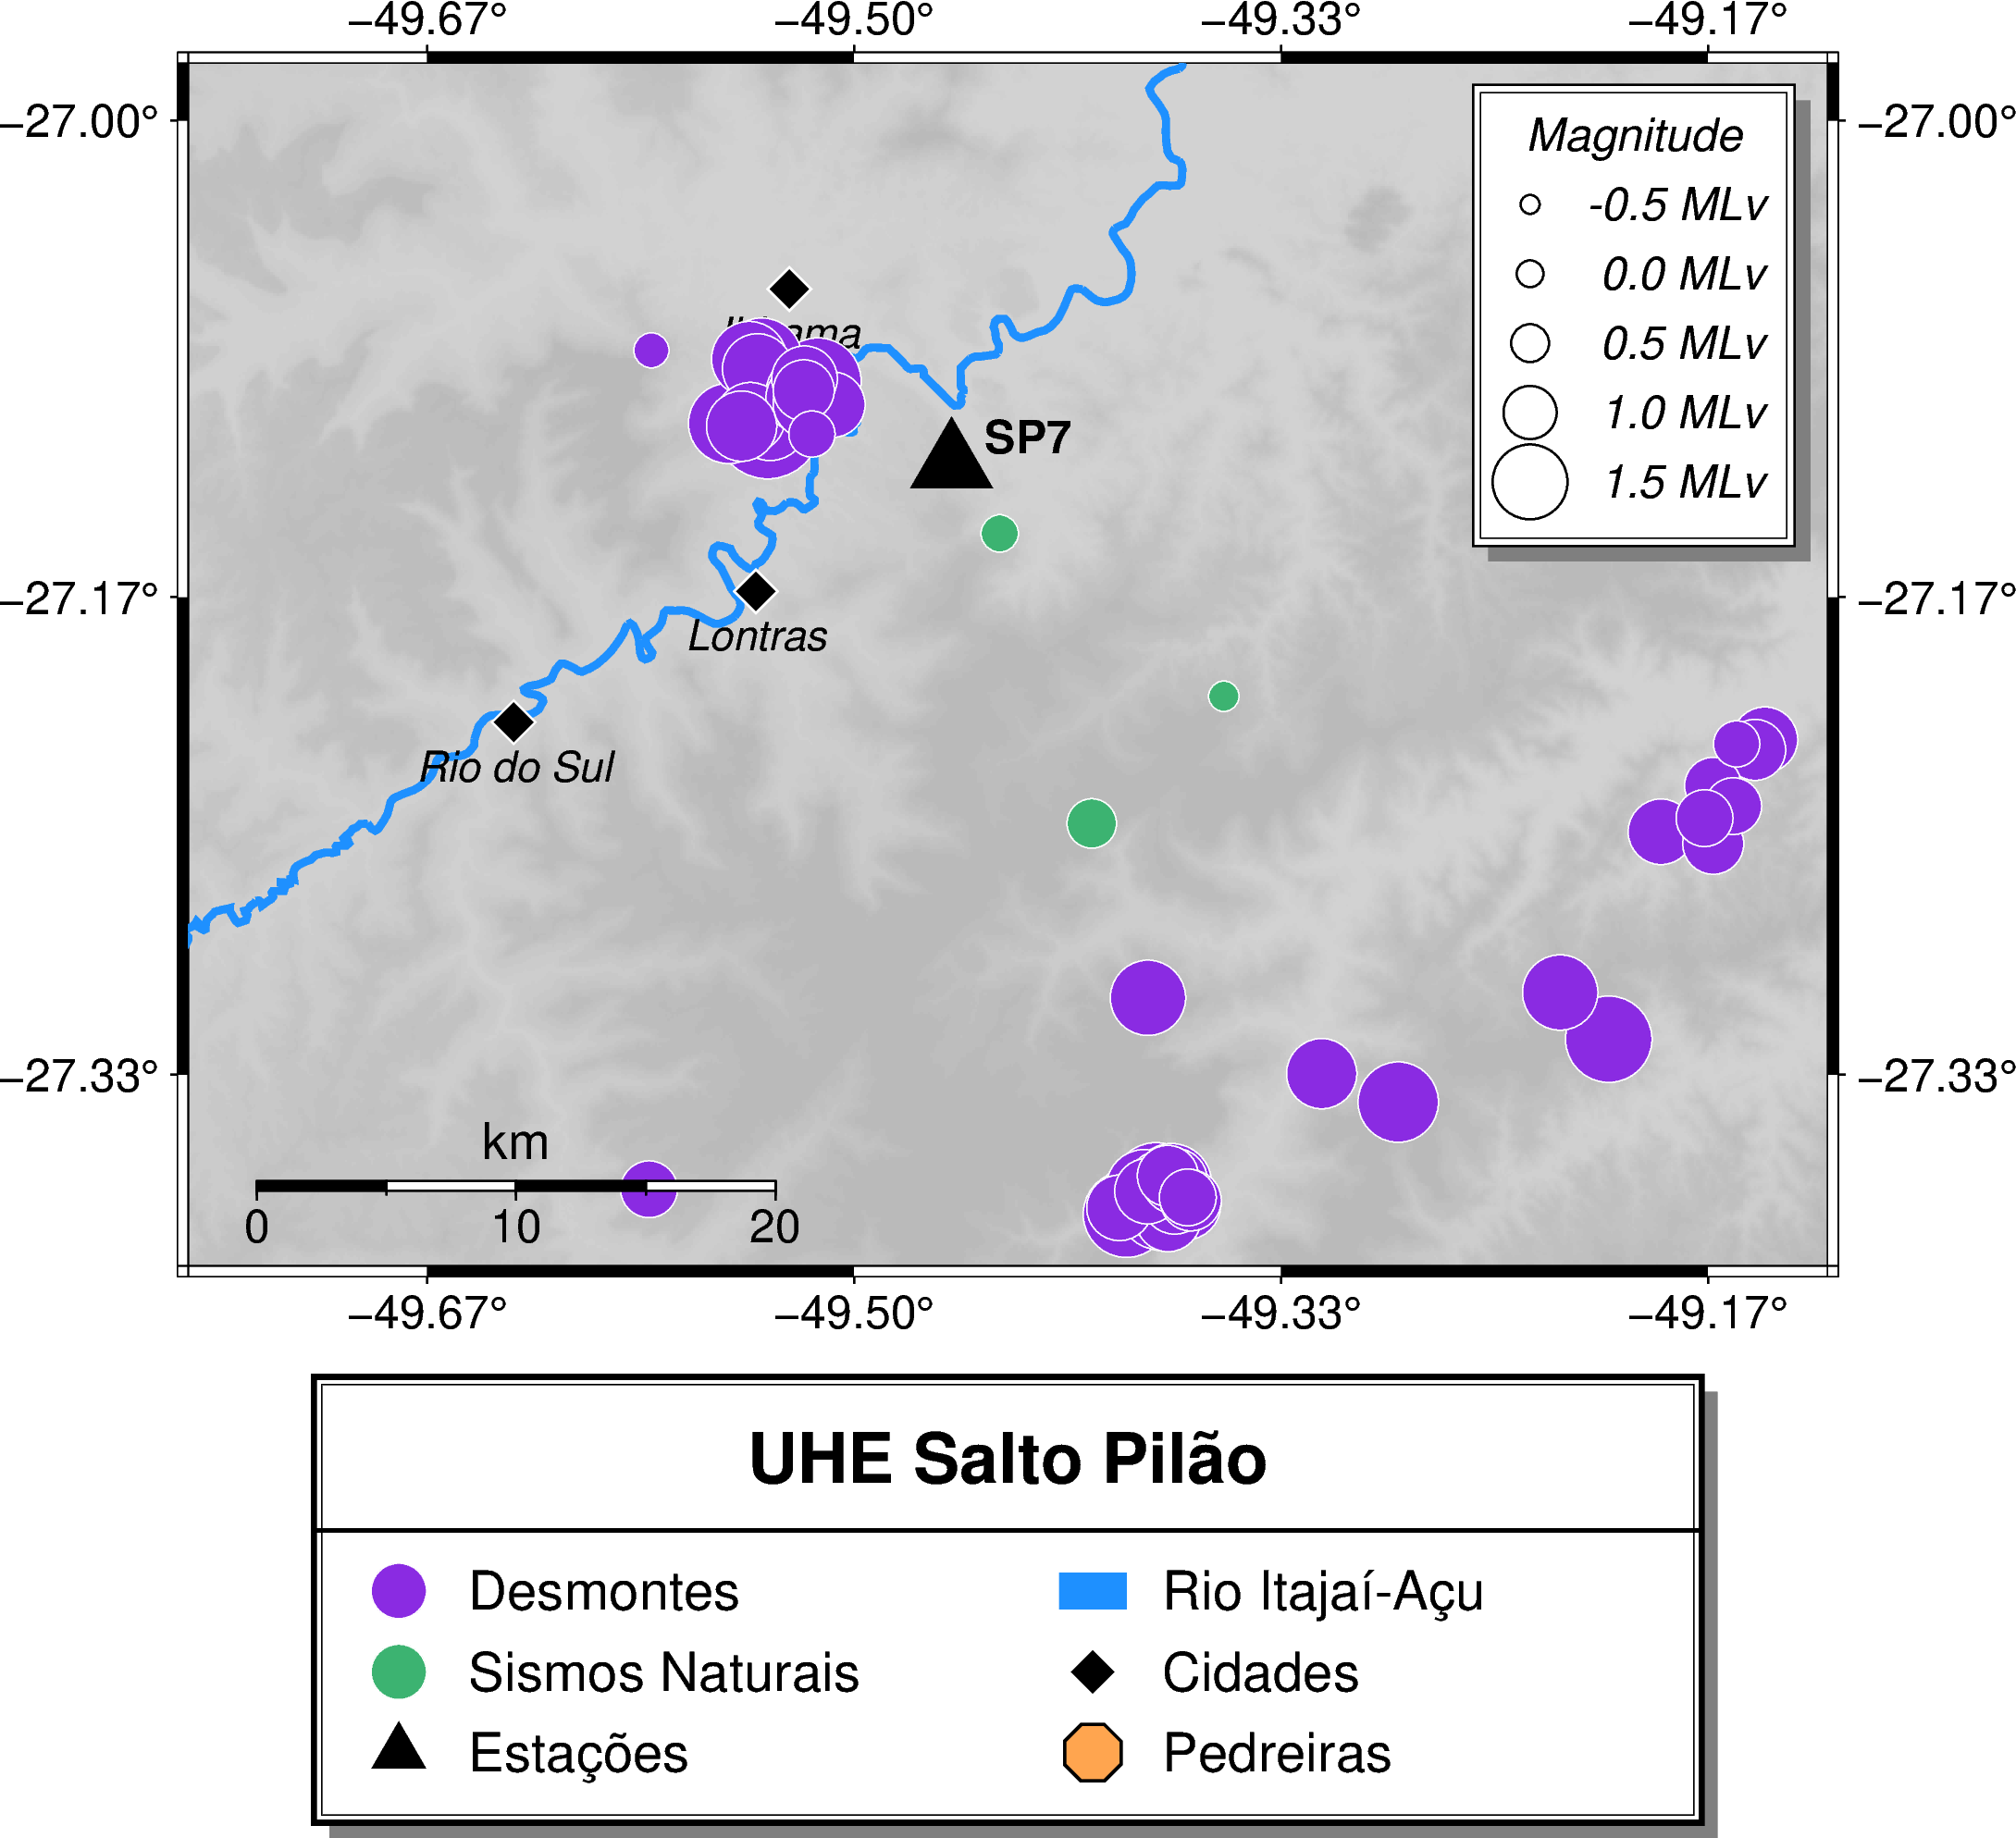
\includegraphics[width=0.8\textwidth]{/home/ggrl/projetos/ClassificadorSismologico/arquivos/figuras/mapas/mapa.png}
    \end{center}
    \end{mdframed}
    \caption*{Fonte: IPT}
\end{figure}


\par{Uma parte significativa do estudo envolveu a análise de eventos sismológicos registrados em horários não comerciais, definidos como o período entre as 23:00 UTC e 11:00 UTC. Este intervalo foi escolhido considerando as diferenças de fuso horário entre as várias regiões do Brasil, que abrangem de -3 UTC a -5 UTC. A análise focou em identificar características distintivas dos eventos naturais e antropogênicos ocorridos neste período.}

\par{Os dados foram processados e visualizados usando uma série de scripts Python desenvolvidos para filtrar, analisar e plotar informações sismológicas detalhadas. Os gráficos resultantes, como distribuições de probabilidade natural, boxplots de distância por natureza do evento e matrizes de correlação, ajudaram a ilustrar diferenças significativas nas características dos eventos registrados durante o horário não comercial.}

\par{Especificamente, a distribuição de \textit{prob\_nat} (probabilidade de um evento ser natural) para eventos naturais mostrou-se distinta daquela para eventos antropogênicos, com eventos naturais tendendo a ter valores mais altos de probabilidade. Além disso, a análise de recall por número de estações envolvidas no registro dos eventos revelou que um maior número de estações frequentemente correlaciona-se a uma classificação mais precisa entre eventos naturais e antropogênicos.}

\par{Os histogramas de recall ajustados para a hora do dia destacaram a precisão da classificação durante os horários não comerciais, refletindo a eficácia do algoritmo em identificar corretamente a natureza dos eventos sob condições variáveis de ruído ambiental e atividade humana.}

\par{Todas essas análises são cruciais para entender a dinâmica sismológica em horários menos típicos para atividades humanas, oferecendo insights sobre a influência de fatores naturais isolados das interferências antrópicas. Os resultados estão detalhados nos Apêndices A e B, onde figuras e tabelas fornecem uma representação visual e quantitativa das descobertas.}

\par{A validação destes resultados foi facilitada pela utilização de scripts automatizados que permitiram uma reprodutibilidade eficiente e a geração de outputs consistentes para análises subsequentes e revisões de estudo.}

\par{Este foco em eventos durante períodos não comerciais não apenas enriquece a compreensão da sismicidade natural mas também aprimora as metodologias de monitoramento e análise sismológica em condições controladas de ruído.}


                    \begin{figure}[H]
                        \centering
<<<<<<< HEAD
                        \includegraphics[width=1.0\textwidth]{/home/ggrl/projetos/ClassificadorSismologico/arquivos/figuras/pos_process/1.54008_boxplot_ev_distance_event.png}
                        \caption{1.54008 boxplot ev distance event}
                        \label{fig:1.54008_boxplot_ev_distance_event}
                    \end{figure}
                

                    \begin{figure}[H]
                        \centering
                        \includegraphics[width=1.0\textwidth]{/home/ggrl/projetos/ClassificadorSismologico/arquivos/figuras/pos_process/n_sta_recall_4.04008.png}
                        \caption{N sta recall 4.04008}
                        \label{fig:n_sta_recall_4.04008}
                    \end{figure}
                

                    \begin{figure}[H]
                        \centering
                        \includegraphics[width=1.0\textwidth]{/home/ggrl/projetos/ClassificadorSismologico/arquivos/figuras/pos_process/n_sta_recall_2.04008.png}
                        \caption{N sta recall 2.04008}
                        \label{fig:n_sta_recall_2.04008}
=======
                        \includegraphics[width=1.0\textwidth]{/home/ipt/projetos/ClassificadorSismologico/arquivos/figuras/pos_processo/dist_snrs.png}
                        \caption{Dist snrs}
                        \label{fig:dist_snrs}
>>>>>>> a17ad66 (commit do ipt)
                    \end{figure}
                

                    \begin{figure}[H]
                        \centering
<<<<<<< HEAD
                        \includegraphics[width=1.0\textwidth]{/home/ggrl/projetos/ClassificadorSismologico/arquivos/figuras/pos_process/n_sta_recall_04008.png}
                        \caption{N sta recall 04008}
                        \label{fig:n_sta_recall_04008}
=======
                        \includegraphics[width=1.0\textwidth]{/home/ipt/projetos/ClassificadorSismologico/arquivos/figuras/pos_processo/mean_snrs_4_prob_nat.png}
                        \caption{Mean snrs 4 prob nat}
                        \label{fig:mean_snrs_4_prob_nat}
>>>>>>> a17ad66 (commit do ipt)
                    \end{figure}
                

                    \begin{figure}[H]
                        \centering
<<<<<<< HEAD
                        \includegraphics[width=1.0\textwidth]{/home/ggrl/projetos/ClassificadorSismologico/arquivos/figuras/pos_process/7.04008_boxplot_ev_distance_event.png}
                        \caption{7.04008 boxplot ev distance event}
                        \label{fig:7.04008_boxplot_ev_distance_event}
=======
                        \includegraphics[width=1.0\textwidth]{/home/ipt/projetos/ClassificadorSismologico/arquivos/figuras/pos_processo/mean_snrs_2.5_prob_nat.png}
                        \caption{Mean snrs 2.5 prob nat}
                        \label{fig:mean_snrs_2.5_prob_nat}
>>>>>>> a17ad66 (commit do ipt)
                    \end{figure}
                

                    \begin{figure}[H]
                        \centering
<<<<<<< HEAD
                        \includegraphics[width=1.0\textwidth]{/home/ggrl/projetos/ClassificadorSismologico/arquivos/figuras/pos_process/04008_hist_ev_distance.png}
                        \caption{04008 hist ev distance}
                        \label{fig:04008_hist_ev_distance}
=======
                        \includegraphics[width=1.0\textwidth]{/home/ipt/projetos/ClassificadorSismologico/arquivos/figuras/pos_processo/mean_snrs_1.25_prob_nat.png}
                        \caption{Mean snrs 1.25 prob nat}
                        \label{fig:mean_snrs_1.25_prob_nat}
>>>>>>> a17ad66 (commit do ipt)
                    \end{figure}
                

                    \begin{figure}[H]
                        \centering
<<<<<<< HEAD
                        \includegraphics[width=1.0\textwidth]{/home/ggrl/projetos/ClassificadorSismologico/arquivos/figuras/pos_process/4.04008_boxplot_ev_distance_event.png}
                        \caption{4.04008 boxplot ev distance event}
                        \label{fig:4.04008_boxplot_ev_distance_event}
=======
                        \includegraphics[width=1.0\textwidth]{/home/ipt/projetos/ClassificadorSismologico/arquivos/figuras/pos_processo/recall_event.png}
                        \caption{Recall event}
                        \label{fig:recall_event}
>>>>>>> a17ad66 (commit do ipt)
                    \end{figure}
                

                    \begin{figure}[H]
                        \centering
<<<<<<< HEAD
                        \includegraphics[width=1.0\textwidth]{/home/ggrl/projetos/ClassificadorSismologico/arquivos/figuras/pos_process/0.754008_boxplot_ev_distance_event.png}
                        \caption{0.754008 boxplot ev distance event}
                        \label{fig:0.754008_boxplot_ev_distance_event}
=======
                        \includegraphics[width=1.0\textwidth]{/home/ipt/projetos/ClassificadorSismologico/arquivos/figuras/pos_processo/mean_snrs_1.5_prob_nat.png}
                        \caption{Mean snrs 1.5 prob nat}
                        \label{fig:mean_snrs_1.5_prob_nat}
                    \end{figure}
                

                    \begin{figure}[H]
                        \centering
                        \includegraphics[width=1.0\textwidth]{/home/ipt/projetos/ClassificadorSismologico/arquivos/figuras/pos_processo/mean_snrs_10_prob_nat.png}
                        \caption{Mean snrs 10 prob nat}
                        \label{fig:mean_snrs_10_prob_nat}
>>>>>>> a17ad66 (commit do ipt)
                    \end{figure}
                

                    \begin{figure}[H]
                        \centering
                        \includegraphics[width=1.0\textwidth]{/home/ggrl/projetos/ClassificadorSismologico/arquivos/figuras/pos_process/5.04008_boxplot_ev_distance_event.png}
                        \caption{5.04008 boxplot ev distance event}
                        \label{fig:5.04008_boxplot_ev_distance_event}
                    \end{figure}
                

                    \begin{figure}[H]
                        \centering
<<<<<<< HEAD
                        \includegraphics[width=1.0\textwidth]{/home/ggrl/projetos/ClassificadorSismologico/arquivos/figuras/pos_process/3.04008_boxplot_ev_distance_event.png}
                        \caption{3.04008 boxplot ev distance event}
                        \label{fig:3.04008_boxplot_ev_distance_event}
                    \end{figure}
                

                    \begin{figure}[H]
                        \centering
                        \includegraphics[width=1.0\textwidth]{/home/ggrl/projetos/ClassificadorSismologico/arquivos/figuras/pos_process/n_sta_recall_0.54008.png}
                        \caption{N sta recall 0.54008}
                        \label{fig:n_sta_recall_0.54008}
=======
                        \includegraphics[width=1.0\textwidth]{/home/ipt/projetos/ClassificadorSismologico/arquivos/figuras/pos_processo/mean_snrs_5_prob_nat.png}
                        \caption{Mean snrs 5 prob nat}
                        \label{fig:mean_snrs_5_prob_nat}
>>>>>>> a17ad66 (commit do ipt)
                    \end{figure}
                

                    \begin{figure}[H]
                        \centering
                        \includegraphics[width=1.0\textwidth]{/home/ggrl/projetos/ClassificadorSismologico/arquivos/figuras/pos_process/04008_boxplot_ev_mag_event.png}
                        \caption{04008 boxplot ev mag event}
                        \label{fig:04008_boxplot_ev_mag_event}
                    \end{figure}
                

                    \begin{figure}[H]
                        \centering
<<<<<<< HEAD
                        \includegraphics[width=1.0\textwidth]{/home/ggrl/projetos/ClassificadorSismologico/arquivos/figuras/pos_process/dist_ev_cat_mag_recall.png}
=======
                        \includegraphics[width=1.0\textwidth]{/home/ipt/projetos/ClassificadorSismologico/arquivos/figuras/pos_processo/hist_ev_distance.png}
                        \caption{Hist ev distance}
                        \label{fig:hist_ev_distance}
                    \end{figure}
                

                    \begin{figure}[H]
                        \centering
                        \includegraphics[width=1.0\textwidth]{/home/ipt/projetos/ClassificadorSismologico/arquivos/figuras/pos_processo/mean_snrs_2_prob_nat.png}
                        \caption{Mean snrs 2 prob nat}
                        \label{fig:mean_snrs_2_prob_nat}
                    \end{figure}
                

                    \begin{figure}[H]
                        \centering
                        \includegraphics[width=1.0\textwidth]{/home/ipt/projetos/ClassificadorSismologico/arquivos/figuras/pos_processo/mean_snrs_6_prob_nat.png}
                        \caption{Mean snrs 6 prob nat}
                        \label{fig:mean_snrs_6_prob_nat}
                    \end{figure}
                

                    \begin{figure}[H]
                        \centering
                        \includegraphics[width=1.0\textwidth]{/home/ipt/projetos/ClassificadorSismologico/arquivos/figuras/pos_processo/mean_snrs_0_prob_nat.png}
                        \caption{Mean snrs 0 prob nat}
                        \label{fig:mean_snrs_0_prob_nat}
                    \end{figure}
                

                    \begin{figure}[H]
                        \centering
                        \includegraphics[width=1.0\textwidth]{/home/ipt/projetos/ClassificadorSismologico/arquivos/figuras/pos_processo/mean_snrs_3_prob_nat.png}
                        \caption{Mean snrs 3 prob nat}
                        \label{fig:mean_snrs_3_prob_nat}
                    \end{figure}
                

                    \begin{figure}[H]
                        \centering
                        \includegraphics[width=1.0\textwidth]{/home/ipt/projetos/ClassificadorSismologico/arquivos/figuras/pos_processo/dist_ev_cat_mag_recall.png}
>>>>>>> a17ad66 (commit do ipt)
                        \caption{Dist ev cat mag recall}
                        \label{fig:dist_ev_cat_mag_recall}
                    \end{figure}
                

                    \begin{figure}[H]
                        \centering
<<<<<<< HEAD
                        \includegraphics[width=1.0\textwidth]{/home/ggrl/projetos/ClassificadorSismologico/arquivos/figuras/pos_process/9.04008_boxplot_ev_distance_event.png}
                        \caption{9.04008 boxplot ev distance event}
                        \label{fig:9.04008_boxplot_ev_distance_event}
=======
                        \includegraphics[width=1.0\textwidth]{/home/ipt/projetos/ClassificadorSismologico/arquivos/figuras/pos_processo/mean_snrs_1.75_prob_nat.png}
                        \caption{Mean snrs 1.75 prob nat}
                        \label{fig:mean_snrs_1.75_prob_nat}
                    \end{figure}
                

                    \begin{figure}[H]
                        \centering
                        \includegraphics[width=1.0\textwidth]{/home/ipt/projetos/ClassificadorSismologico/arquivos/figuras/pos_processo/dist_ev_num_stations_recall.png}
                        \caption{Dist ev num stations recall}
                        \label{fig:dist_ev_num_stations_recall}
>>>>>>> a17ad66 (commit do ipt)
                    \end{figure}
                

                    \begin{figure}[H]
                        \centering
                        \includegraphics[width=1.0\textwidth]{/home/ggrl/projetos/ClassificadorSismologico/arquivos/figuras/pos_process/n_sta_recall_1.254008.png}
                        \caption{N sta recall 1.254008}
                        \label{fig:n_sta_recall_1.254008}
                    \end{figure}
                

                    \begin{figure}[H]
                        \centering
<<<<<<< HEAD
                        \includegraphics[width=1.0\textwidth]{/home/ggrl/projetos/ClassificadorSismologico/arquivos/figuras/pos_process/n_sta_recall_1.54008.png}
                        \caption{N sta recall 1.54008}
                        \label{fig:n_sta_recall_1.54008}
                    \end{figure}
                

                    \begin{figure}[H]
                        \centering
                        \includegraphics[width=1.0\textwidth]{/home/ggrl/projetos/ClassificadorSismologico/arquivos/figuras/pos_process/1.04008_boxplot_ev_distance_event.png}
                        \caption{1.04008 boxplot ev distance event}
                        \label{fig:1.04008_boxplot_ev_distance_event}
                    \end{figure}
                

                    \begin{figure}[H]
                        \centering
                        \includegraphics[width=1.0\textwidth]{/home/ggrl/projetos/ClassificadorSismologico/arquivos/figuras/pos_process/04008_dist_mean_snrs_recall.png}
                        \caption{04008 dist mean snrs recall}
                        \label{fig:04008_dist_mean_snrs_recall}
                    \end{figure}
                

                    \begin{figure}[H]
                        \centering
                        \includegraphics[width=1.0\textwidth]{/home/ggrl/projetos/ClassificadorSismologico/arquivos/figuras/pos_process/1.254008_boxplot_ev_distance_event.png}
                        \caption{1.254008 boxplot ev distance event}
                        \label{fig:1.254008_boxplot_ev_distance_event}
                    \end{figure}
                

                    \begin{figure}[H]
                        \centering
                        \includegraphics[width=1.0\textwidth]{/home/ggrl/projetos/ClassificadorSismologico/arquivos/figuras/pos_process/2.04008_boxplot_ev_distance_event.png}
                        \caption{2.04008 boxplot ev distance event}
                        \label{fig:2.04008_boxplot_ev_distance_event}
                    \end{figure}
                

                    \begin{figure}[H]
                        \centering
                        \includegraphics[width=1.0\textwidth]{/home/ggrl/projetos/ClassificadorSismologico/arquivos/figuras/pos_process/04008_hist_ev_distance_event.png}
                        \caption{04008 hist ev distance event}
                        \label{fig:04008_hist_ev_distance_event}
                    \end{figure}
                

                    \begin{figure}[H]
                        \centering
                        \includegraphics[width=1.0\textwidth]{/home/ggrl/projetos/ClassificadorSismologico/arquivos/figuras/pos_process/n_sta_recall_1.754008.png}
                        \caption{N sta recall 1.754008}
                        \label{fig:n_sta_recall_1.754008}
                    \end{figure}
                

                    \begin{figure}[H]
                        \centering
                        \includegraphics[width=1.0\textwidth]{/home/ggrl/projetos/ClassificadorSismologico/arquivos/figuras/pos_process/hist_ev_hour_recall_event.png}
                        \caption{Hist ev hour recall event}
                        \label{fig:hist_ev_hour_recall_event}
                    \end{figure}
                

                    \begin{figure}[H]
                        \centering
                        \includegraphics[width=1.0\textwidth]{/home/ggrl/projetos/ClassificadorSismologico/arquivos/figuras/pos_process/8.04008_boxplot_ev_distance_event.png}
                        \caption{8.04008 boxplot ev distance event}
                        \label{fig:8.04008_boxplot_ev_distance_event}
                    \end{figure}
                

                    \begin{figure}[H]
                        \centering
                        \includegraphics[width=1.0\textwidth]{/home/ggrl/projetos/ClassificadorSismologico/arquivos/figuras/pos_process/04008_boxplot_ev_distance_event.png}
                        \caption{04008 boxplot ev distance event}
                        \label{fig:04008_boxplot_ev_distance_event}
                    \end{figure}
                

                    \begin{figure}[H]
                        \centering
                        \includegraphics[width=1.0\textwidth]{/home/ggrl/projetos/ClassificadorSismologico/arquivos/figuras/pos_process/n_sta_recall_3.04008.png}
                        \caption{N sta recall 3.04008}
                        \label{fig:n_sta_recall_3.04008}
                    \end{figure}
                

                    \begin{figure}[H]
                        \centering
                        \includegraphics[width=1.0\textwidth]{/home/ggrl/projetos/ClassificadorSismologico/arquivos/figuras/pos_process/1.754008_boxplot_ev_distance_event.png}
                        \caption{1.754008 boxplot ev distance event}
                        \label{fig:1.754008_boxplot_ev_distance_event}
                    \end{figure}
                

                    \begin{figure}[H]
                        \centering
                        \includegraphics[width=1.0\textwidth]{/home/ggrl/projetos/ClassificadorSismologico/arquivos/figuras/pos_process/n_sta_recall_1.04008.png}
                        \caption{N sta recall 1.04008}
                        \label{fig:n_sta_recall_1.04008}
                    \end{figure}
                

                    \begin{figure}[H]
                        \centering
                        \includegraphics[width=1.0\textwidth]{/home/ggrl/projetos/ClassificadorSismologico/arquivos/figuras/pos_process/n_sta_recall_0.254008.png}
                        \caption{N sta recall 0.254008}
                        \label{fig:n_sta_recall_0.254008}
                    \end{figure}
                

                    \begin{figure}[H]
                        \centering
                        \includegraphics[width=1.0\textwidth]{/home/ggrl/projetos/ClassificadorSismologico/arquivos/figuras/pos_process/dist_snrs_recall.png}
                        \caption{Dist snrs recall}
                        \label{fig:dist_snrs_recall}
                    \end{figure}
                

                    \begin{figure}[H]
                        \centering
                        \includegraphics[width=1.0\textwidth]{/home/ggrl/projetos/ClassificadorSismologico/arquivos/figuras/pos_process/n_sta_recall_0.754008.png}
                        \caption{N sta recall 0.754008}
                        \label{fig:n_sta_recall_0.754008}
                    \end{figure}
                

                    \begin{figure}[H]
                        \centering
                        \includegraphics[width=1.0\textwidth]{/home/ggrl/projetos/ClassificadorSismologico/arquivos/figuras/pos_process/region_corr.png}
=======
                        \includegraphics[width=1.0\textwidth]{/home/ipt/projetos/ClassificadorSismologico/arquivos/figuras/pos_processo/region_corr.png}
>>>>>>> a17ad66 (commit do ipt)
                        \caption{Region corr}
                        \label{fig:region_corr}
                    \end{figure}
                

                    \begin{figure}[H]
                        \centering
<<<<<<< HEAD
                        \includegraphics[width=1.0\textwidth]{/home/ggrl/projetos/ClassificadorSismologico/arquivos/figuras/pos_process/10.04008_boxplot_ev_distance_event.png}
                        \caption{10.04008 boxplot ev distance event}
                        \label{fig:10.04008_boxplot_ev_distance_event}
                    \end{figure}
                

                    \begin{figure}[H]
                        \centering
                        \includegraphics[width=1.0\textwidth]{/home/ggrl/projetos/ClassificadorSismologico/arquivos/figuras/pos_process/6.04008_boxplot_ev_distance_event.png}
                        \caption{6.04008 boxplot ev distance event}
                        \label{fig:6.04008_boxplot_ev_distance_event}
                    \end{figure}
                

                    \begin{figure}[H]
                        \centering
                        \includegraphics[width=1.0\textwidth]{/home/ggrl/projetos/ClassificadorSismologico/arquivos/figuras/pos_process/0.254008_boxplot_ev_distance_event.png}
                        \caption{0.254008 boxplot ev distance event}
                        \label{fig:0.254008_boxplot_ev_distance_event}
                    \end{figure}
                

                    \begin{figure}[H]
                        \centering
                        \includegraphics[width=1.0\textwidth]{/home/ggrl/projetos/ClassificadorSismologico/arquivos/figuras/pos_process/0.54008_boxplot_ev_distance_event.png}
                        \caption{0.54008 boxplot ev distance event}
                        \label{fig:0.54008_boxplot_ev_distance_event}
                    \end{figure}
                

                    \begin{figure}[H]
                        \centering
                        \includegraphics[width=1.0\textwidth]{/home/ggrl/projetos/ClassificadorSismologico/arquivos/figuras/pos_process/plots/.bkp/boxplot_XV.png}
                        \caption{Boxplot xv}
                        \label{fig:boxplot_XV}
                    \end{figure}
                

                    \begin{figure}[H]
                        \centering
                        \includegraphics[width=1.0\textwidth]{/home/ggrl/projetos/ClassificadorSismologico/arquivos/figuras/pos_process/plots/.bkp/boxplot_BL.png}
                        \caption{Boxplot bl}
                        \label{fig:boxplot_BL}
                    \end{figure}
                

                    \begin{figure}[H]
                        \centering
                        \includegraphics[width=1.0\textwidth]{/home/ggrl/projetos/ClassificadorSismologico/arquivos/figuras/pos_process/plots/.bkp/boxplot_ON.png}
                        \caption{Boxplot on}
                        \label{fig:boxplot_ON}
                    \end{figure}
                

                    \begin{figure}[H]
                        \centering
                        \includegraphics[width=1.0\textwidth]{/home/ggrl/projetos/ClassificadorSismologico/arquivos/figuras/pos_process/plots/.bkp/dist_ev_num_stations_recall.png}
                        \caption{Dist ev num stations recall}
                        \label{fig:dist_ev_num_stations_recall}
=======
                        \includegraphics[width=1.0\textwidth]{/home/ipt/projetos/ClassificadorSismologico/arquivos/figuras/pos_processo/dist_prob_nat.png}
                        \caption{Dist prob nat}
                        \label{fig:dist_prob_nat}
>>>>>>> a17ad66 (commit do ipt)
                    \end{figure}
                

                    \begin{figure}[H]
                        \centering
<<<<<<< HEAD
                        \includegraphics[width=1.0\textwidth]{/home/ggrl/projetos/ClassificadorSismologico/arquivos/figuras/pos_process/plots/.bkp/boxplot_NB.png}
                        \caption{Boxplot nb}
                        \label{fig:boxplot_NB}
                    \end{figure}
                

                    \begin{figure}[H]
                        \centering
                        \includegraphics[width=1.0\textwidth]{/home/ggrl/projetos/ClassificadorSismologico/arquivos/figuras/pos_process/plots/.bkp/boxplot_rede.png}
                        \caption{Boxplot rede}
                        \label{fig:boxplot_rede}
                    \end{figure}
                

                    \begin{figure}[H]
                        \centering
                        \includegraphics[width=1.0\textwidth]{/home/ggrl/projetos/ClassificadorSismologico/arquivos/figuras/pos_process/plots/.bkp/dist_ev_cat_mag_recall.png}
                        \caption{Dist ev cat mag recall}
                        \label{fig:dist_ev_cat_mag_recall}
                    \end{figure}
                

                    \begin{figure}[H]
                        \centering
                        \includegraphics[width=1.0\textwidth]{/home/ggrl/projetos/ClassificadorSismologico/arquivos/figuras/pos_process/plots/.bkp/hist_ev_distance.png}
                        \caption{Hist ev distance}
                        \label{fig:hist_ev_distance}
                    \end{figure}
                

                    \begin{figure}[H]
                        \centering
                        \includegraphics[width=1.0\textwidth]{/home/ggrl/projetos/ClassificadorSismologico/arquivos/figuras/pos_process/plots/.bkp/boxplot_BR.png}
                        \caption{Boxplot br}
                        \label{fig:boxplot_BR}
                    \end{figure}
                

                    \begin{figure}[H]
                        \centering
                        \includegraphics[width=1.0\textwidth]{/home/ggrl/projetos/ClassificadorSismologico/arquivos/figuras/pos_process/plots/.bkp/boxplot_XC.png}
                        \caption{Boxplot xc}
                        \label{fig:boxplot_XC}
                    \end{figure}
                

                    \begin{figure}[H]
                        \centering
                        \includegraphics[width=1.0\textwidth]{/home/ggrl/projetos/ClassificadorSismologico/arquivos/figuras/pos_process/plots/.bkp/boxplot_IM.png}
                        \caption{Boxplot im}
                        \label{fig:boxplot_IM}
                    \end{figure}
                

                    \begin{figure}[H]
                        \centering
                        \includegraphics[width=1.0\textwidth]{/home/ggrl/projetos/ClassificadorSismologico/arquivos/figuras/pos_process/plots/.bkp/boxplot_Y4.png}
                        \caption{Boxplot y4}
                        \label{fig:boxplot_Y4}
                    \end{figure}
                

                    \begin{figure}[H]
                        \centering
                        \includegraphics[width=1.0\textwidth]{/home/ggrl/projetos/ClassificadorSismologico/arquivos/figuras/pos_process/plots/.bkp/dist_prob_nat_recall.png}
                        \caption{Dist prob nat recall}
                        \label{fig:dist_prob_nat_recall}
                    \end{figure}
                

                    \begin{figure}[H]
                        \centering
                        \includegraphics[width=1.0\textwidth]{/home/ggrl/projetos/ClassificadorSismologico/arquivos/figuras/pos_process/plots/.bkp/boxplot_BX.png}
                        \caption{Boxplot bx}
                        \label{fig:boxplot_BX}
                    \end{figure}
                

                    \begin{figure}[H]
                        \centering
                        \includegraphics[width=1.0\textwidth]{/home/ggrl/projetos/ClassificadorSismologico/arquivos/figuras/pos_process/plots/.bkp/dist_snrs_recall.png}
                        \caption{Dist snrs recall}
                        \label{fig:dist_snrs_recall}
                    \end{figure}
                

                    \begin{figure}[H]
                        \centering
                        \includegraphics[width=1.0\textwidth]{/home/ggrl/projetos/ClassificadorSismologico/arquivos/figuras/pos_process/plots/.bkp/boxplot_VL.png}
                        \caption{Boxplot vl}
                        \label{fig:boxplot_VL}
                    \end{figure}
                

                    \begin{figure}[H]
                        \centering
                        \includegraphics[width=1.0\textwidth]{/home/ggrl/projetos/ClassificadorSismologico/arquivos/figuras/pos_process/plots/.bkp/hist_ev_hour_recall.png}
                        \caption{Hist ev hour recall}
                        \label{fig:hist_ev_hour_recall}
                    \end{figure}
                

                    \begin{figure}[H]
                        \centering
                        \includegraphics[width=1.0\textwidth]{/home/ggrl/projetos/ClassificadorSismologico/arquivos/figuras/pos_process/plots/.bkp/boxplot_GT.png}
                        \caption{Boxplot gt}
                        \label{fig:boxplot_GT}
                    \end{figure}
                

                    \begin{figure}[H]
                        \centering
                        \includegraphics[width=1.0\textwidth]{/home/ggrl/projetos/ClassificadorSismologico/arquivos/figuras/pos_process/plots/.bkp/boxplot_dist.png}
                        \caption{Boxplot dist}
                        \label{fig:boxplot_dist}
                    \end{figure}
                

                    \begin{figure}[H]
                        \centering
                        \includegraphics[width=1.0\textwidth]{/home/ggrl/projetos/ClassificadorSismologico/arquivos/figuras/pos_process/plots/.bkp/region_corr.png}
                        \caption{Region corr}
                        \label{fig:region_corr}
                    \end{figure}
                

                    \begin{figure}[H]
                        \centering
                        \includegraphics[width=1.0\textwidth]{/home/ggrl/projetos/ClassificadorSismologico/arquivos/figuras/pos_process/.bkp/1.54008_boxplot_ev_distance_event.png}
                        \caption{1.54008 boxplot ev distance event}
                        \label{fig:1.54008_boxplot_ev_distance_event}
                    \end{figure}
                

                    \begin{figure}[H]
                        \centering
                        \includegraphics[width=1.0\textwidth]{/home/ggrl/projetos/ClassificadorSismologico/arquivos/figuras/pos_process/.bkp/n_sta_recall_4.04008.png}
                        \caption{N sta recall 4.04008}
                        \label{fig:n_sta_recall_4.04008}
                    \end{figure}
                

                    \begin{figure}[H]
                        \centering
                        \includegraphics[width=1.0\textwidth]{/home/ggrl/projetos/ClassificadorSismologico/arquivos/figuras/pos_process/.bkp/n_sta_recall_5.04008.png}
                        \caption{N sta recall 5.04008}
                        \label{fig:n_sta_recall_5.04008}
                    \end{figure}
                

                    \begin{figure}[H]
                        \centering
                        \includegraphics[width=1.0\textwidth]{/home/ggrl/projetos/ClassificadorSismologico/arquivos/figuras/pos_process/.bkp/n_sta_recall_2.04008.png}
                        \caption{N sta recall 2.04008}
                        \label{fig:n_sta_recall_2.04008}
                    \end{figure}
                

                    \begin{figure}[H]
                        \centering
                        \includegraphics[width=1.0\textwidth]{/home/ggrl/projetos/ClassificadorSismologico/arquivos/figuras/pos_process/.bkp/boxplot_XV.png}
                        \caption{Boxplot xv}
                        \label{fig:boxplot_XV}
                    \end{figure}
                

                    \begin{figure}[H]
                        \centering
                        \includegraphics[width=1.0\textwidth]{/home/ggrl/projetos/ClassificadorSismologico/arquivos/figuras/pos_process/.bkp/11.04008_boxplot_ev_distance_event.png}
                        \caption{11.04008 boxplot ev distance event}
                        \label{fig:11.04008_boxplot_ev_distance_event}
                    \end{figure}
                

                    \begin{figure}[H]
                        \centering
                        \includegraphics[width=1.0\textwidth]{/home/ggrl/projetos/ClassificadorSismologico/arquivos/figuras/pos_process/.bkp/boxplot_BL.png}
                        \caption{Boxplot bl}
                        \label{fig:boxplot_BL}
                    \end{figure}
                

                    \begin{figure}[H]
                        \centering
                        \includegraphics[width=1.0\textwidth]{/home/ggrl/projetos/ClassificadorSismologico/arquivos/figuras/pos_process/.bkp/n_sta_recall_9.04008.png}
                        \caption{N sta recall 9.04008}
                        \label{fig:n_sta_recall_9.04008}
                    \end{figure}
                

                    \begin{figure}[H]
                        \centering
                        \includegraphics[width=1.0\textwidth]{/home/ggrl/projetos/ClassificadorSismologico/arquivos/figuras/pos_process/.bkp/boxplot_ON.png}
                        \caption{Boxplot on}
                        \label{fig:boxplot_ON}
                    \end{figure}
                

                    \begin{figure}[H]
                        \centering
                        \includegraphics[width=1.0\textwidth]{/home/ggrl/projetos/ClassificadorSismologico/arquivos/figuras/pos_process/.bkp/n_sta_recall_04008.png}
                        \caption{N sta recall 04008}
                        \label{fig:n_sta_recall_04008}
                    \end{figure}
                

                    \begin{figure}[H]
                        \centering
                        \includegraphics[width=1.0\textwidth]{/home/ggrl/projetos/ClassificadorSismologico/arquivos/figuras/pos_process/.bkp/7.04008_boxplot_ev_distance_event.png}
                        \caption{7.04008 boxplot ev distance event}
                        \label{fig:7.04008_boxplot_ev_distance_event}
                    \end{figure}
                

                    \begin{figure}[H]
                        \centering
                        \includegraphics[width=1.0\textwidth]{/home/ggrl/projetos/ClassificadorSismologico/arquivos/figuras/pos_process/.bkp/104008_boxplot_ev_mag_event.png}
                        \caption{104008 boxplot ev mag event}
                        \label{fig:104008_boxplot_ev_mag_event}
                    \end{figure}
                

                    \begin{figure}[H]
                        \centering
                        \includegraphics[width=1.0\textwidth]{/home/ggrl/projetos/ClassificadorSismologico/arquivos/figuras/pos_process/.bkp/n_sta_recall_5.54008.png}
                        \caption{N sta recall 5.54008}
                        \label{fig:n_sta_recall_5.54008}
                    \end{figure}
                

                    \begin{figure}[H]
                        \centering
                        \includegraphics[width=1.0\textwidth]{/home/ggrl/projetos/ClassificadorSismologico/arquivos/figuras/pos_process/.bkp/n_sta_recall_84008.png}
                        \caption{N sta recall 84008}
                        \label{fig:n_sta_recall_84008}
                    \end{figure}
                

                    \begin{figure}[H]
                        \centering
                        \includegraphics[width=1.0\textwidth]{/home/ggrl/projetos/ClassificadorSismologico/arquivos/figuras/pos_process/.bkp/n_sta_recall_8.04008.png}
                        \caption{N sta recall 8.04008}
                        \label{fig:n_sta_recall_8.04008}
                    \end{figure}
                

                    \begin{figure}[H]
                        \centering
                        \includegraphics[width=1.0\textwidth]{/home/ggrl/projetos/ClassificadorSismologico/arquivos/figuras/pos_process/.bkp/dist_ev_num_stations_recall.png}
                        \caption{Dist ev num stations recall}
                        \label{fig:dist_ev_num_stations_recall}
                    \end{figure}
                

                    \begin{figure}[H]
                        \centering
                        \includegraphics[width=1.0\textwidth]{/home/ggrl/projetos/ClassificadorSismologico/arquivos/figuras/pos_process/.bkp/boxplot_UY.png}
                        \caption{Boxplot uy}
                        \label{fig:boxplot_UY}
                    \end{figure}
                

                    \begin{figure}[H]
                        \centering
                        \includegraphics[width=1.0\textwidth]{/home/ggrl/projetos/ClassificadorSismologico/arquivos/figuras/pos_process/.bkp/104004_boxplot_ev_mag_event.png}
                        \caption{104004 boxplot ev mag event}
                        \label{fig:104004_boxplot_ev_mag_event}
                    \end{figure}
                

                    \begin{figure}[H]
                        \centering
                        \includegraphics[width=1.0\textwidth]{/home/ggrl/projetos/ClassificadorSismologico/arquivos/figuras/pos_process/.bkp/n_sta_recall_204008.png}
                        \caption{N sta recall 204008}
                        \label{fig:n_sta_recall_204008}
                    \end{figure}
                

                    \begin{figure}[H]
                        \centering
                        \includegraphics[width=1.0\textwidth]{/home/ggrl/projetos/ClassificadorSismologico/arquivos/figuras/pos_process/.bkp/4.04008_boxplot_ev_distance_event.png}
                        \caption{4.04008 boxplot ev distance event}
                        \label{fig:4.04008_boxplot_ev_distance_event}
                    \end{figure}
                

                    \begin{figure}[H]
                        \centering
                        \includegraphics[width=1.0\textwidth]{/home/ggrl/projetos/ClassificadorSismologico/arquivos/figuras/pos_process/.bkp/14008_dist_mean_snrs_recall.png}
                        \caption{14008 dist mean snrs recall}
                        \label{fig:14008_dist_mean_snrs_recall}
                    \end{figure}
                

                    \begin{figure}[H]
                        \centering
                        \includegraphics[width=1.0\textwidth]{/home/ggrl/projetos/ClassificadorSismologico/arquivos/figuras/pos_process/.bkp/34008_boxplot_ev_distance_event.png}
                        \caption{34008 boxplot ev distance event}
                        \label{fig:34008_boxplot_ev_distance_event}
                    \end{figure}
                

                    \begin{figure}[H]
                        \centering
                        \includegraphics[width=1.0\textwidth]{/home/ggrl/projetos/ClassificadorSismologico/arquivos/figuras/pos_process/.bkp/n_sta_recall_3.54008.png}
                        \caption{N sta recall 3.54008}
                        \label{fig:n_sta_recall_3.54008}
                    \end{figure}
                

                    \begin{figure}[H]
                        \centering
                        \includegraphics[width=1.0\textwidth]{/home/ggrl/projetos/ClassificadorSismologico/arquivos/figuras/pos_process/.bkp/n_sta_recall_2504.png}
                        \caption{N sta recall 2504}
                        \label{fig:n_sta_recall_2504}
                    \end{figure}
                

                    \begin{figure}[H]
                        \centering
                        \includegraphics[width=1.0\textwidth]{/home/ggrl/projetos/ClassificadorSismologico/arquivos/figuras/pos_process/.bkp/54004_boxplot_ev_distance_event.png}
                        \caption{54004 boxplot ev distance event}
                        \label{fig:54004_boxplot_ev_distance_event}
                    \end{figure}
                

                    \begin{figure}[H]
                        \centering
                        \includegraphics[width=1.0\textwidth]{/home/ggrl/projetos/ClassificadorSismologico/arquivos/figuras/pos_process/.bkp/34004_boxplot_ev_distance_event.png}
                        \caption{34004 boxplot ev distance event}
                        \label{fig:34004_boxplot_ev_distance_event}
                    \end{figure}
                

                    \begin{figure}[H]
                        \centering
                        \includegraphics[width=1.0\textwidth]{/home/ggrl/projetos/ClassificadorSismologico/arquivos/figuras/pos_process/.bkp/0.754008_boxplot_ev_distance_event.png}
                        \caption{0.754008 boxplot ev distance event}
                        \label{fig:0.754008_boxplot_ev_distance_event}
                    \end{figure}
                

                    \begin{figure}[H]
                        \centering
                        \includegraphics[width=1.0\textwidth]{/home/ggrl/projetos/ClassificadorSismologico/arquivos/figuras/pos_process/.bkp/dist_ev_cat_mag.png}
                        \caption{Dist ev cat mag}
                        \label{fig:dist_ev_cat_mag}
                    \end{figure}
                

                    \begin{figure}[H]
                        \centering
                        \includegraphics[width=1.0\textwidth]{/home/ggrl/projetos/ClassificadorSismologico/arquivos/figuras/pos_process/.bkp/204004_boxplot_ev_distance_event.png}
                        \caption{204004 boxplot ev distance event}
                        \label{fig:204004_boxplot_ev_distance_event}
                    \end{figure}
                

                    \begin{figure}[H]
                        \centering
                        \includegraphics[width=1.0\textwidth]{/home/ggrl/projetos/ClassificadorSismologico/arquivos/figuras/pos_process/.bkp/dist_ev_num_stations_absoluto.png}
                        \caption{Dist ev num stations absoluto}
                        \label{fig:dist_ev_num_stations_absoluto}
                    \end{figure}
                

                    \begin{figure}[H]
                        \centering
                        \includegraphics[width=1.0\textwidth]{/home/ggrl/projetos/ClassificadorSismologico/arquivos/figuras/pos_process/.bkp/n_sta_recall_94008.png}
                        \caption{N sta recall 94008}
                        \label{fig:n_sta_recall_94008}
                    \end{figure}
                

                    \begin{figure}[H]
                        \centering
                        \includegraphics[width=1.0\textwidth]{/home/ggrl/projetos/ClassificadorSismologico/arquivos/figuras/pos_process/.bkp/boxplot_NB.png}
                        \caption{Boxplot nb}
                        \label{fig:boxplot_NB}
                    \end{figure}
                

                    \begin{figure}[H]
                        \centering
                        \includegraphics[width=1.0\textwidth]{/home/ggrl/projetos/ClassificadorSismologico/arquivos/figuras/pos_process/.bkp/14004_boxplot_ev_distance_event.png}
                        \caption{14004 boxplot ev distance event}
                        \label{fig:14004_boxplot_ev_distance_event}
                    \end{figure}
                

                    \begin{figure}[H]
                        \centering
                        \includegraphics[width=1.0\textwidth]{/home/ggrl/projetos/ClassificadorSismologico/arquivos/figuras/pos_process/.bkp/5.04008_boxplot_ev_distance_event.png}
                        \caption{5.04008 boxplot ev distance event}
                        \label{fig:5.04008_boxplot_ev_distance_event}
                    \end{figure}
                

                    \begin{figure}[H]
                        \centering
                        \includegraphics[width=1.0\textwidth]{/home/ggrl/projetos/ClassificadorSismologico/arquivos/figuras/pos_process/.bkp/24008_boxplot_ev_distance_event.png}
                        \caption{24008 boxplot ev distance event}
                        \label{fig:24008_boxplot_ev_distance_event}
                    \end{figure}
                

                    \begin{figure}[H]
                        \centering
                        \includegraphics[width=1.0\textwidth]{/home/ggrl/projetos/ClassificadorSismologico/arquivos/figuras/pos_process/.bkp/3.04008_boxplot_ev_distance_event.png}
                        \caption{3.04008 boxplot ev distance event}
                        \label{fig:3.04008_boxplot_ev_distance_event}
                    \end{figure}
                

                    \begin{figure}[H]
                        \centering
                        \includegraphics[width=1.0\textwidth]{/home/ggrl/projetos/ClassificadorSismologico/arquivos/figuras/pos_process/.bkp/boxplot_rede.png}
                        \caption{Boxplot rede}
                        \label{fig:boxplot_rede}
                    \end{figure}
                

                    \begin{figure}[H]
                        \centering
                        \includegraphics[width=1.0\textwidth]{/home/ggrl/projetos/ClassificadorSismologico/arquivos/figuras/pos_process/.bkp/1snr_boxplot_ev_distance_event.png}
                        \caption{1snr boxplot ev distance event}
                        \label{fig:1snr_boxplot_ev_distance_event}
                    \end{figure}
                

                    \begin{figure}[H]
                        \centering
                        \includegraphics[width=1.0\textwidth]{/home/ggrl/projetos/ClassificadorSismologico/arquivos/figuras/pos_process/.bkp/04004_boxplot_ev_distance_event.png}
                        \caption{04004 boxplot ev distance event}
                        \label{fig:04004_boxplot_ev_distance_event}
                    \end{figure}
                

                    \begin{figure}[H]
                        \centering
                        \includegraphics[width=1.0\textwidth]{/home/ggrl/projetos/ClassificadorSismologico/arquivos/figuras/pos_process/.bkp/33504_boxplot_ev_distance_event.png}
                        \caption{33504 boxplot ev distance event}
                        \label{fig:33504_boxplot_ev_distance_event}
                    \end{figure}
                

                    \begin{figure}[H]
                        \centering
                        \includegraphics[width=1.0\textwidth]{/home/ggrl/projetos/ClassificadorSismologico/arquivos/figuras/pos_process/.bkp/n_sta_recall_0.54008.png}
                        \caption{N sta recall 0.54008}
                        \label{fig:n_sta_recall_0.54008}
                    \end{figure}
                

                    \begin{figure}[H]
                        \centering
                        \includegraphics[width=1.0\textwidth]{/home/ggrl/projetos/ClassificadorSismologico/arquivos/figuras/pos_process/.bkp/n_sta_recall_3.754008.png}
                        \caption{N sta recall 3.754008}
                        \label{fig:n_sta_recall_3.754008}
                    \end{figure}
                

                    \begin{figure}[H]
                        \centering
                        \includegraphics[width=1.0\textwidth]{/home/ggrl/projetos/ClassificadorSismologico/arquivos/figuras/pos_process/.bkp/04008_boxplot_ev_mag_event.png}
                        \caption{04008 boxplot ev mag event}
                        \label{fig:04008_boxplot_ev_mag_event}
                    \end{figure}
                

                    \begin{figure}[H]
                        \centering
                        \includegraphics[width=1.0\textwidth]{/home/ggrl/projetos/ClassificadorSismologico/arquivos/figuras/pos_process/.bkp/dist_mean_snrs_recall.png}
                        \caption{Dist mean snrs recall}
                        \label{fig:dist_mean_snrs_recall}
                    \end{figure}
                

                    \begin{figure}[H]
                        \centering
                        \includegraphics[width=1.0\textwidth]{/home/ggrl/projetos/ClassificadorSismologico/arquivos/figuras/pos_process/.bkp/dist_ev_cat_mag_recall.png}
                        \caption{Dist ev cat mag recall}
                        \label{fig:dist_ev_cat_mag_recall}
                    \end{figure}
                

                    \begin{figure}[H]
                        \centering
                        \includegraphics[width=1.0\textwidth]{/home/ggrl/projetos/ClassificadorSismologico/arquivos/figuras/pos_process/.bkp/hist_ev_distance.png}
                        \caption{Hist ev distance}
                        \label{fig:hist_ev_distance}
                    \end{figure}
                

                    \begin{figure}[H]
                        \centering
                        \includegraphics[width=1.0\textwidth]{/home/ggrl/projetos/ClassificadorSismologico/arquivos/figuras/pos_process/.bkp/n_sta_recall_154008.png}
                        \caption{N sta recall 154008}
                        \label{fig:n_sta_recall_154008}
                    \end{figure}
                

                    \begin{figure}[H]
                        \centering
                        \includegraphics[width=1.0\textwidth]{/home/ggrl/projetos/ClassificadorSismologico/arquivos/figuras/pos_process/.bkp/n_sta_recall_254008.png}
                        \caption{N sta recall 254008}
                        \label{fig:n_sta_recall_254008}
                    \end{figure}
                

                    \begin{figure}[H]
                        \centering
                        \includegraphics[width=1.0\textwidth]{/home/ggrl/projetos/ClassificadorSismologico/arquivos/figuras/pos_process/.bkp/9.04008_boxplot_ev_distance_event.png}
                        \caption{9.04008 boxplot ev distance event}
                        \label{fig:9.04008_boxplot_ev_distance_event}
                    \end{figure}
                

                    \begin{figure}[H]
                        \centering
                        \includegraphics[width=1.0\textwidth]{/home/ggrl/projetos/ClassificadorSismologico/arquivos/figuras/pos_process/.bkp/n_sta_recall_24008.png}
                        \caption{N sta recall 24008}
                        \label{fig:n_sta_recall_24008}
                    \end{figure}
                

                    \begin{figure}[H]
                        \centering
                        \includegraphics[width=1.0\textwidth]{/home/ggrl/projetos/ClassificadorSismologico/arquivos/figuras/pos_process/.bkp/n_sta_recall_54008.png}
                        \caption{N sta recall 54008}
                        \label{fig:n_sta_recall_54008}
                    \end{figure}
                

                    \begin{figure}[H]
                        \centering
                        \includegraphics[width=1.0\textwidth]{/home/ggrl/projetos/ClassificadorSismologico/arquivos/figuras/pos_process/.bkp/n_sta_recall_2.254008.png}
                        \caption{N sta recall 2.254008}
                        \label{fig:n_sta_recall_2.254008}
                    \end{figure}
                

                    \begin{figure}[H]
                        \centering
                        \includegraphics[width=1.0\textwidth]{/home/ggrl/projetos/ClassificadorSismologico/arquivos/figuras/pos_process/.bkp/n_sta_recall_14008.png}
                        \caption{N sta recall 14008}
                        \label{fig:n_sta_recall_14008}
                    \end{figure}
                

                    \begin{figure}[H]
                        \centering
                        \includegraphics[width=1.0\textwidth]{/home/ggrl/projetos/ClassificadorSismologico/arquivos/figuras/pos_process/.bkp/hist_hora.png}
                        \caption{Hist hora}
                        \label{fig:hist_hora}
                    \end{figure}
                

                    \begin{figure}[H]
                        \centering
                        \includegraphics[width=1.0\textwidth]{/home/ggrl/projetos/ClassificadorSismologico/arquivos/figuras/pos_process/.bkp/n_sta_recall_1.254008.png}
                        \caption{N sta recall 1.254008}
                        \label{fig:n_sta_recall_1.254008}
                    \end{figure}
                

                    \begin{figure}[H]
                        \centering
                        \includegraphics[width=1.0\textwidth]{/home/ggrl/projetos/ClassificadorSismologico/arquivos/figuras/pos_process/.bkp/boxplot_BR.png}
                        \caption{Boxplot br}
                        \label{fig:boxplot_BR}
                    \end{figure}
                

                    \begin{figure}[H]
                        \centering
                        \includegraphics[width=1.0\textwidth]{/home/ggrl/projetos/ClassificadorSismologico/arquivos/figuras/pos_process/.bkp/34008_dist_mean_snrs_recall.png}
                        \caption{34008 dist mean snrs recall}
                        \label{fig:34008_dist_mean_snrs_recall}
                    \end{figure}
                

                    \begin{figure}[H]
                        \centering
                        \includegraphics[width=1.0\textwidth]{/home/ggrl/projetos/ClassificadorSismologico/arquivos/figuras/pos_process/.bkp/n_sta_recall_3.254008.png}
                        \caption{N sta recall 3.254008}
                        \label{fig:n_sta_recall_3.254008}
                    \end{figure}
                

                    \begin{figure}[H]
                        \centering
                        \includegraphics[width=1.0\textwidth]{/home/ggrl/projetos/ClassificadorSismologico/arquivos/figuras/pos_process/.bkp/dist_ev_distance_rel_freq.png}
                        \caption{Dist ev distance rel freq}
                        \label{fig:dist_ev_distance_rel_freq}
                    \end{figure}
                

                    \begin{figure}[H]
                        \centering
                        \includegraphics[width=1.0\textwidth]{/home/ggrl/projetos/ClassificadorSismologico/arquivos/figuras/pos_process/.bkp/24008_dist_mean_snrs_recall.png}
                        \caption{24008 dist mean snrs recall}
                        \label{fig:24008_dist_mean_snrs_recall}
                    \end{figure}
                

                    \begin{figure}[H]
                        \centering
                        \includegraphics[width=1.0\textwidth]{/home/ggrl/projetos/ClassificadorSismologico/arquivos/figuras/pos_process/.bkp/n_sta_recall_1.54008.png}
                        \caption{N sta recall 1.54008}
                        \label{fig:n_sta_recall_1.54008}
                    \end{figure}
                

                    \begin{figure}[H]
                        \centering
                        \includegraphics[width=1.0\textwidth]{/home/ggrl/projetos/ClassificadorSismologico/arquivos/figuras/pos_process/.bkp/14008_boxplot_ev_distance_event.png}
                        \caption{14008 boxplot ev distance event}
                        \label{fig:14008_boxplot_ev_distance_event}
                    \end{figure}
                

                    \begin{figure}[H]
                        \centering
                        \includegraphics[width=1.0\textwidth]{/home/ggrl/projetos/ClassificadorSismologico/arquivos/figuras/pos_process/.bkp/n_sta_recall_44008.png}
                        \caption{N sta recall 44008}
                        \label{fig:n_sta_recall_44008}
                    \end{figure}
                

                    \begin{figure}[H]
                        \centering
                        \includegraphics[width=1.0\textwidth]{/home/ggrl/projetos/ClassificadorSismologico/arquivos/figuras/pos_process/.bkp/0snr_boxplot_ev_distance_event.png}
                        \caption{0snr boxplot ev distance event}
                        \label{fig:0snr_boxplot_ev_distance_event}
                    \end{figure}
                

                    \begin{figure}[H]
                        \centering
                        \includegraphics[width=1.0\textwidth]{/home/ggrl/projetos/ClassificadorSismologico/arquivos/figuras/pos_process/.bkp/n_sta_recall_4.754008.png}
                        \caption{N sta recall 4.754008}
                        \label{fig:n_sta_recall_4.754008}
                    \end{figure}
                

                    \begin{figure}[H]
                        \centering
                        \includegraphics[width=1.0\textwidth]{/home/ggrl/projetos/ClassificadorSismologico/arquivos/figuras/pos_process/.bkp/n_sta_recall_104008.png}
                        \caption{N sta recall 104008}
                        \label{fig:n_sta_recall_104008}
                    \end{figure}
                

                    \begin{figure}[H]
                        \centering
                        \includegraphics[width=1.0\textwidth]{/home/ggrl/projetos/ClassificadorSismologico/arquivos/figuras/pos_process/.bkp/n_sta_recall_2.754008.png}
                        \caption{N sta recall 2.754008}
                        \label{fig:n_sta_recall_2.754008}
                    \end{figure}
                

                    \begin{figure}[H]
                        \centering
                        \includegraphics[width=1.0\textwidth]{/home/ggrl/projetos/ClassificadorSismologico/arquivos/figuras/pos_process/.bkp/boxplot_XC.png}
                        \caption{Boxplot xc}
                        \label{fig:boxplot_XC}
                    \end{figure}
                

                    \begin{figure}[H]
                        \centering
                        \includegraphics[width=1.0\textwidth]{/home/ggrl/projetos/ClassificadorSismologico/arquivos/figuras/pos_process/.bkp/24004_boxplot_ev_mag_event.png}
                        \caption{24004 boxplot ev mag event}
                        \label{fig:24004_boxplot_ev_mag_event}
                    \end{figure}
                

                    \begin{figure}[H]
                        \centering
                        \includegraphics[width=1.0\textwidth]{/home/ggrl/projetos/ClassificadorSismologico/arquivos/figuras/pos_process/.bkp/mean_snrs_0_prob_nat.png}
                        \caption{Mean snrs 0 prob nat}
                        \label{fig:mean_snrs_0_prob_nat}
                    \end{figure}
                

                    \begin{figure}[H]
                        \centering
                        \includegraphics[width=1.0\textwidth]{/home/ggrl/projetos/ClassificadorSismologico/arquivos/figuras/pos_process/.bkp/104004_boxplot_ev_distance_event.png}
                        \caption{104004 boxplot ev distance event}
                        \label{fig:104004_boxplot_ev_distance_event}
                    \end{figure}
                

                    \begin{figure}[H]
                        \centering
                        \includegraphics[width=1.0\textwidth]{/home/ggrl/projetos/ClassificadorSismologico/arquivos/figuras/pos_process/.bkp/n_sta_recall_5.754008.png}
                        \caption{N sta recall 5.754008}
                        \label{fig:n_sta_recall_5.754008}
                    \end{figure}
                

                    \begin{figure}[H]
                        \centering
                        \includegraphics[width=1.0\textwidth]{/home/ggrl/projetos/ClassificadorSismologico/arquivos/figuras/pos_process/.bkp/n_sta_recall_6.04008.png}
                        \caption{N sta recall 6.04008}
                        \label{fig:n_sta_recall_6.04008}
                    \end{figure}
                

                    \begin{figure}[H]
                        \centering
                        \includegraphics[width=1.0\textwidth]{/home/ggrl/projetos/ClassificadorSismologico/arquivos/figuras/pos_process/.bkp/dist_snrs.png}
                        \caption{Dist snrs}
                        \label{fig:dist_snrs}
                    \end{figure}
                

                    \begin{figure}[H]
                        \centering
                        \includegraphics[width=1.0\textwidth]{/home/ggrl/projetos/ClassificadorSismologico/arquivos/figuras/pos_process/.bkp/1.04008_boxplot_ev_distance_event.png}
                        \caption{1.04008 boxplot ev distance event}
                        \label{fig:1.04008_boxplot_ev_distance_event}
                    \end{figure}
                

                    \begin{figure}[H]
                        \centering
                        \includegraphics[width=1.0\textwidth]{/home/ggrl/projetos/ClassificadorSismologico/arquivos/figuras/pos_process/.bkp/04008_dist_mean_snrs_recall.png}
                        \caption{04008 dist mean snrs recall}
                        \label{fig:04008_dist_mean_snrs_recall}
                    \end{figure}
                

                    \begin{figure}[H]
                        \centering
                        \includegraphics[width=1.0\textwidth]{/home/ggrl/projetos/ClassificadorSismologico/arquivos/figuras/pos_process/.bkp/n_sta_recall_24004.png}
                        \caption{N sta recall 24004}
                        \label{fig:n_sta_recall_24004}
                    \end{figure}
                

                    \begin{figure}[H]
                        \centering
                        \includegraphics[width=1.0\textwidth]{/home/ggrl/projetos/ClassificadorSismologico/arquivos/figuras/pos_process/.bkp/104008_boxplot_ev_distance_event.png}
                        \caption{104008 boxplot ev distance event}
                        \label{fig:104008_boxplot_ev_distance_event}
                    \end{figure}
                

                    \begin{figure}[H]
                        \centering
                        \includegraphics[width=1.0\textwidth]{/home/ggrl/projetos/ClassificadorSismologico/arquivos/figuras/pos_process/.bkp/24008_boxplot_ev_mag_event.png}
                        \caption{24008 boxplot ev mag event}
                        \label{fig:24008_boxplot_ev_mag_event}
                    \end{figure}
                

                    \begin{figure}[H]
                        \centering
                        \includegraphics[width=1.0\textwidth]{/home/ggrl/projetos/ClassificadorSismologico/arquivos/figuras/pos_process/.bkp/hist_ev_hour_recall_pick.png}
                        \caption{Hist ev hour recall pick}
                        \label{fig:hist_ev_hour_recall_pick}
                    \end{figure}
                

                    \begin{figure}[H]
                        \centering
                        \includegraphics[width=1.0\textwidth]{/home/ggrl/projetos/ClassificadorSismologico/arquivos/figuras/pos_process/.bkp/n_sta_recall_64008.png}
                        \caption{N sta recall 64008}
                        \label{fig:n_sta_recall_64008}
                    \end{figure}
                

                    \begin{figure}[H]
                        \centering
                        \includegraphics[width=1.0\textwidth]{/home/ggrl/projetos/ClassificadorSismologico/arquivos/figuras/pos_process/.bkp/1.254008_boxplot_ev_distance_event.png}
                        \caption{1.254008 boxplot ev distance event}
                        \label{fig:1.254008_boxplot_ev_distance_event}
                    \end{figure}
                

                    \begin{figure}[H]
                        \centering
                        \includegraphics[width=1.0\textwidth]{/home/ggrl/projetos/ClassificadorSismologico/arquivos/figuras/pos_process/.bkp/2.04008_boxplot_ev_distance_event.png}
                        \caption{2.04008 boxplot ev distance event}
                        \label{fig:2.04008_boxplot_ev_distance_event}
                    \end{figure}
                

                    \begin{figure}[H]
                        \centering
                        \includegraphics[width=1.0\textwidth]{/home/ggrl/projetos/ClassificadorSismologico/arquivos/figuras/pos_process/.bkp/boxplot_BV.png}
                        \caption{Boxplot bv}
                        \label{fig:boxplot_BV}
                    \end{figure}
                

                    \begin{figure}[H]
                        \centering
                        \includegraphics[width=1.0\textwidth]{/home/ggrl/projetos/ClassificadorSismologico/arquivos/figuras/pos_process/.bkp/n_sta_recall_1.754008.png}
                        \caption{N sta recall 1.754008}
                        \label{fig:n_sta_recall_1.754008}
                    \end{figure}
                

                    \begin{figure}[H]
                        \centering
                        \includegraphics[width=1.0\textwidth]{/home/ggrl/projetos/ClassificadorSismologico/arquivos/figuras/pos_process/.bkp/dist_prob_nat.png}
                        \caption{Dist prob nat}
                        \label{fig:dist_prob_nat}
                    \end{figure}
                

                    \begin{figure}[H]
                        \centering
                        \includegraphics[width=1.0\textwidth]{/home/ggrl/projetos/ClassificadorSismologico/arquivos/figuras/pos_process/.bkp/hist_ev_hour_recall_event.png}
                        \caption{Hist ev hour recall event}
                        \label{fig:hist_ev_hour_recall_event}
                    \end{figure}
                

                    \begin{figure}[H]
                        \centering
                        \includegraphics[width=1.0\textwidth]{/home/ggrl/projetos/ClassificadorSismologico/arquivos/figuras/pos_process/.bkp/boxplot_IM.png}
                        \caption{Boxplot im}
                        \label{fig:boxplot_IM}
                    \end{figure}
                

                    \begin{figure}[H]
                        \centering
                        \includegraphics[width=1.0\textwidth]{/home/ggrl/projetos/ClassificadorSismologico/arquivos/figuras/pos_process/.bkp/53504_boxplot_ev_distance_event.png}
                        \caption{53504 boxplot ev distance event}
                        \label{fig:53504_boxplot_ev_distance_event}
                    \end{figure}
                

                    \begin{figure}[H]
                        \centering
                        \includegraphics[width=1.0\textwidth]{/home/ggrl/projetos/ClassificadorSismologico/arquivos/figuras/pos_process/.bkp/8.04008_boxplot_ev_distance_event.png}
                        \caption{8.04008 boxplot ev distance event}
                        \label{fig:8.04008_boxplot_ev_distance_event}
                    \end{figure}
                

                    \begin{figure}[H]
                        \centering
                        \includegraphics[width=1.0\textwidth]{/home/ggrl/projetos/ClassificadorSismologico/arquivos/figuras/pos_process/.bkp/boxplot_ev_distance_event.png}
                        \caption{Boxplot ev distance event}
                        \label{fig:boxplot_ev_distance_event}
                    \end{figure}
                

                    \begin{figure}[H]
                        \centering
                        \includegraphics[width=1.0\textwidth]{/home/ggrl/projetos/ClassificadorSismologico/arquivos/figuras/pos_process/.bkp/24004_boxplot_ev_distance_event.png}
                        \caption{24004 boxplot ev distance event}
                        \label{fig:24004_boxplot_ev_distance_event}
                    \end{figure}
                

                    \begin{figure}[H]
                        \centering
                        \includegraphics[width=1.0\textwidth]{/home/ggrl/projetos/ClassificadorSismologico/arquivos/figuras/pos_process/.bkp/44004_boxplot_ev_distance_event.png}
                        \caption{44004 boxplot ev distance event}
                        \label{fig:44004_boxplot_ev_distance_event}
                    \end{figure}
                

                    \begin{figure}[H]
                        \centering
                        \includegraphics[width=1.0\textwidth]{/home/ggrl/projetos/ClassificadorSismologico/arquivos/figuras/pos_process/.bkp/dist_ev_num_stations_recall_pick.png}
                        \caption{Dist ev num stations recall pick}
                        \label{fig:dist_ev_num_stations_recall_pick}
                    \end{figure}
                

                    \begin{figure}[H]
                        \centering
                        \includegraphics[width=1.0\textwidth]{/home/ggrl/projetos/ClassificadorSismologico/arquivos/figuras/pos_process/.bkp/boxplot_Y4.png}
                        \caption{Boxplot y4}
                        \label{fig:boxplot_Y4}
                    \end{figure}
                

                    \begin{figure}[H]
                        \centering
                        \includegraphics[width=1.0\textwidth]{/home/ggrl/projetos/ClassificadorSismologico/arquivos/figuras/pos_process/.bkp/04008_boxplot_ev_distance_event.png}
                        \caption{04008 boxplot ev distance event}
                        \label{fig:04008_boxplot_ev_distance_event}
                    \end{figure}
                

                    \begin{figure}[H]
                        \centering
                        \includegraphics[width=1.0\textwidth]{/home/ggrl/projetos/ClassificadorSismologico/arquivos/figuras/pos_process/.bkp/n_sta_recall_7.04008.png}
                        \caption{N sta recall 7.04008}
                        \label{fig:n_sta_recall_7.04008}
                    \end{figure}
                

                    \begin{figure}[H]
                        \centering
                        \includegraphics[width=1.0\textwidth]{/home/ggrl/projetos/ClassificadorSismologico/arquivos/figuras/pos_process/.bkp/54008_boxplot_ev_distance_event.png}
                        \caption{54008 boxplot ev distance event}
                        \label{fig:54008_boxplot_ev_distance_event}
                    \end{figure}
                

                    \begin{figure}[H]
                        \centering
                        \includegraphics[width=1.0\textwidth]{/home/ggrl/projetos/ClassificadorSismologico/arquivos/figuras/pos_process/.bkp/n_sta_recall_3.04008.png}
                        \caption{N sta recall 3.04008}
                        \label{fig:n_sta_recall_3.04008}
                    \end{figure}
                

                    \begin{figure}[H]
                        \centering
                        \includegraphics[width=1.0\textwidth]{/home/ggrl/projetos/ClassificadorSismologico/arquivos/figuras/pos_process/.bkp/recall_event.png}
                        \caption{Recall event}
                        \label{fig:recall_event}
                    \end{figure}
                

                    \begin{figure}[H]
                        \centering
                        \includegraphics[width=1.0\textwidth]{/home/ggrl/projetos/ClassificadorSismologico/arquivos/figuras/pos_process/.bkp/mean_snrs_1_prob_nat.png}
=======
                        \includegraphics[width=1.0\textwidth]{/home/ipt/projetos/ClassificadorSismologico/arquivos/figuras/pos_processo/mean_snrs_1_prob_nat.png}
>>>>>>> a17ad66 (commit do ipt)
                        \caption{Mean snrs 1 prob nat}
                        \label{fig:mean_snrs_1_prob_nat}
                    \end{figure}
                

                    \begin{figure}[H]
                        \centering
<<<<<<< HEAD
                        \includegraphics[width=1.0\textwidth]{/home/ggrl/projetos/ClassificadorSismologico/arquivos/figuras/pos_process/.bkp/1.754008_boxplot_ev_distance_event.png}
                        \caption{1.754008 boxplot ev distance event}
                        \label{fig:1.754008_boxplot_ev_distance_event}
                    \end{figure}
                

                    \begin{figure}[H]
                        \centering
                        \includegraphics[width=1.0\textwidth]{/home/ggrl/projetos/ClassificadorSismologico/arquivos/figuras/pos_process/.bkp/boxplot_BX.png}
                        \caption{Boxplot bx}
                        \label{fig:boxplot_BX}
                    \end{figure}
                

                    \begin{figure}[H]
                        \centering
                        \includegraphics[width=1.0\textwidth]{/home/ggrl/projetos/ClassificadorSismologico/arquivos/figuras/pos_process/.bkp/n_sta_recall_34008.png}
                        \caption{N sta recall 34008}
                        \label{fig:n_sta_recall_34008}
                    \end{figure}
                

                    \begin{figure}[H]
                        \centering
                        \includegraphics[width=1.0\textwidth]{/home/ggrl/projetos/ClassificadorSismologico/arquivos/figuras/pos_process/.bkp/12.04008_boxplot_ev_distance_event.png}
                        \caption{12.04008 boxplot ev distance event}
                        \label{fig:12.04008_boxplot_ev_distance_event}
                    \end{figure}
                

                    \begin{figure}[H]
                        \centering
                        \includegraphics[width=1.0\textwidth]{/home/ggrl/projetos/ClassificadorSismologico/arquivos/figuras/pos_process/.bkp/n_sta_recall_124008.png}
                        \caption{N sta recall 124008}
                        \label{fig:n_sta_recall_124008}
                    \end{figure}
                

                    \begin{figure}[H]
                        \centering
                        \includegraphics[width=1.0\textwidth]{/home/ggrl/projetos/ClassificadorSismologico/arquivos/figuras/pos_process/.bkp/4008_recall_event.png}
                        \caption{4008 recall event}
                        \label{fig:4008_recall_event}
                    \end{figure}
                

                    \begin{figure}[H]
                        \centering
                        \includegraphics[width=1.0\textwidth]{/home/ggrl/projetos/ClassificadorSismologico/arquivos/figuras/pos_process/.bkp/scatter_snrs_prob_nat.png}
                        \caption{Scatter snrs prob nat}
                        \label{fig:scatter_snrs_prob_nat}
                    \end{figure}
                

                    \begin{figure}[H]
                        \centering
                        \includegraphics[width=1.0\textwidth]{/home/ggrl/projetos/ClassificadorSismologico/arquivos/figuras/pos_process/.bkp/n_sta_recall_74008.png}
                        \caption{N sta recall 74008}
                        \label{fig:n_sta_recall_74008}
                    \end{figure}
                

                    \begin{figure}[H]
                        \centering
                        \includegraphics[width=1.0\textwidth]{/home/ggrl/projetos/ClassificadorSismologico/arquivos/figuras/pos_process/.bkp/hist_ev_distance_event.png}
                        \caption{Hist ev distance event}
                        \label{fig:hist_ev_distance_event}
                    \end{figure}
                

                    \begin{figure}[H]
                        \centering
                        \includegraphics[width=1.0\textwidth]{/home/ggrl/projetos/ClassificadorSismologico/arquivos/figuras/pos_process/.bkp/1.754004_boxplot_ev_distance_event.png}
                        \caption{1.754004 boxplot ev distance event}
                        \label{fig:1.754004_boxplot_ev_distance_event}
                    \end{figure}
                

                    \begin{figure}[H]
                        \centering
                        \includegraphics[width=1.0\textwidth]{/home/ggrl/projetos/ClassificadorSismologico/arquivos/figuras/pos_process/.bkp/n_sta_recall_1.04008.png}
                        \caption{N sta recall 1.04008}
                        \label{fig:n_sta_recall_1.04008}
                    \end{figure}
                

                    \begin{figure}[H]
                        \centering
                        \includegraphics[width=1.0\textwidth]{/home/ggrl/projetos/ClassificadorSismologico/arquivos/figuras/pos_process/.bkp/n_sta_recall_4.54008.png}
                        \caption{N sta recall 4.54008}
                        \label{fig:n_sta_recall_4.54008}
                    \end{figure}
                

                    \begin{figure}[H]
                        \centering
                        \includegraphics[width=1.0\textwidth]{/home/ggrl/projetos/ClassificadorSismologico/arquivos/figuras/pos_process/.bkp/n_sta_recall_0.254008.png}
                        \caption{N sta recall 0.254008}
                        \label{fig:n_sta_recall_0.254008}
                    \end{figure}
                

                    \begin{figure}[H]
                        \centering
                        \includegraphics[width=1.0\textwidth]{/home/ggrl/projetos/ClassificadorSismologico/arquivos/figuras/pos_process/.bkp/dist_snrs_recall.png}
                        \caption{Dist snrs recall}
                        \label{fig:dist_snrs_recall}
                    \end{figure}
                

                    \begin{figure}[H]
                        \centering
                        \includegraphics[width=1.0\textwidth]{/home/ggrl/projetos/ClassificadorSismologico/arquivos/figuras/pos_process/.bkp/1.94004_boxplot_ev_distance_event.png}
                        \caption{1.94004 boxplot ev distance event}
                        \label{fig:1.94004_boxplot_ev_distance_event}
                    \end{figure}
                

                    \begin{figure}[H]
                        \centering
                        \includegraphics[width=1.0\textwidth]{/home/ggrl/projetos/ClassificadorSismologico/arquivos/figuras/pos_process/.bkp/boxplot_VL.png}
                        \caption{Boxplot vl}
                        \label{fig:boxplot_VL}
                    \end{figure}
                

                    \begin{figure}[H]
                        \centering
                        \includegraphics[width=1.0\textwidth]{/home/ggrl/projetos/ClassificadorSismologico/arquivos/figuras/pos_process/.bkp/n_sta_recall_0.754008.png}
                        \caption{N sta recall 0.754008}
                        \label{fig:n_sta_recall_0.754008}
                    \end{figure}
                

                    \begin{figure}[H]
                        \centering
                        \includegraphics[width=1.0\textwidth]{/home/ggrl/projetos/ClassificadorSismologico/arquivos/figuras/pos_process/.bkp/hist_ev_hour_recall.png}
                        \caption{Hist ev hour recall}
                        \label{fig:hist_ev_hour_recall}
                    \end{figure}
                

                    \begin{figure}[H]
                        \centering
                        \includegraphics[width=1.0\textwidth]{/home/ggrl/projetos/ClassificadorSismologico/arquivos/figuras/pos_process/.bkp/boxplot_GT.png}
                        \caption{Boxplot gt}
                        \label{fig:boxplot_GT}
=======
                        \includegraphics[width=1.0\textwidth]{/home/ipt/projetos/ClassificadorSismologico/arquivos/figuras/pos_processo/hist_prob_nat.png}
                        \caption{Hist prob nat}
                        \label{fig:hist_prob_nat}
>>>>>>> a17ad66 (commit do ipt)
                    \end{figure}
                

                    \begin{figure}[H]
                        \centering
                        \includegraphics[width=1.0\textwidth]{/home/ggrl/projetos/ClassificadorSismologico/arquivos/figuras/pos_process/.bkp/boxplot_dist.png}
                        \caption{Boxplot dist}
                        \label{fig:boxplot_dist}
                    \end{figure}
                

                    \begin{figure}[H]
                        \centering
                        \includegraphics[width=1.0\textwidth]{/home/ggrl/projetos/ClassificadorSismologico/arquivos/figuras/pos_process/.bkp/region_corr.png}
                        \caption{Region corr}
                        \label{fig:region_corr}
                    \end{figure}
                

                    \begin{figure}[H]
                        \centering
                        \includegraphics[width=1.0\textwidth]{/home/ggrl/projetos/ClassificadorSismologico/arquivos/figuras/pos_process/.bkp/n_sta_recall_10.04008.png}
                        \caption{N sta recall 10.04008}
                        \label{fig:n_sta_recall_10.04008}
                    \end{figure}
                

                    \begin{figure}[H]
                        \centering
                        \includegraphics[width=1.0\textwidth]{/home/ggrl/projetos/ClassificadorSismologico/arquivos/figuras/pos_process/.bkp/n_sta_recall_2.54008.png}
                        \caption{N sta recall 2.54008}
                        \label{fig:n_sta_recall_2.54008}
                    \end{figure}
                

                    \begin{figure}[H]
                        \centering
                        \includegraphics[width=1.0\textwidth]{/home/ggrl/projetos/ClassificadorSismologico/arquivos/figuras/pos_process/.bkp/10.04008_boxplot_ev_distance_event.png}
                        \caption{10.04008 boxplot ev distance event}
                        \label{fig:10.04008_boxplot_ev_distance_event}
                    \end{figure}
                

                    \begin{figure}[H]
                        \centering
                        \includegraphics[width=1.0\textwidth]{/home/ggrl/projetos/ClassificadorSismologico/arquivos/figuras/pos_process/.bkp/6.04008_boxplot_ev_distance_event.png}
                        \caption{6.04008 boxplot ev distance event}
                        \label{fig:6.04008_boxplot_ev_distance_event}
                    \end{figure}
                

                    \begin{figure}[H]
                        \centering
                        \includegraphics[width=1.0\textwidth]{/home/ggrl/projetos/ClassificadorSismologico/arquivos/figuras/pos_process/.bkp/n_sta_recall_4.254008.png}
                        \caption{N sta recall 4.254008}
                        \label{fig:n_sta_recall_4.254008}
                    \end{figure}
                

                    \begin{figure}[H]
                        \centering
                        \includegraphics[width=1.0\textwidth]{/home/ggrl/projetos/ClassificadorSismologico/arquivos/figuras/pos_process/.bkp/dist_ev_num_stations_recall_event.png}
                        \caption{Dist ev num stations recall event}
                        \label{fig:dist_ev_num_stations_recall_event}
                    \end{figure}
                

                    \begin{figure}[H]
                        \centering
                        \includegraphics[width=1.0\textwidth]{/home/ggrl/projetos/ClassificadorSismologico/arquivos/figuras/pos_process/.bkp/0.254008_boxplot_ev_distance_event.png}
                        \caption{0.254008 boxplot ev distance event}
                        \label{fig:0.254008_boxplot_ev_distance_event}
                    \end{figure}
                

                    \begin{figure}[H]
                        \centering
                        \includegraphics[width=1.0\textwidth]{/home/ggrl/projetos/ClassificadorSismologico/arquivos/figuras/pos_process/.bkp/corr_matrix.png}
                        \caption{Corr matrix}
                        \label{fig:corr_matrix}
                    \end{figure}
                

                    \begin{figure}[H]
                        \centering
                        \includegraphics[width=1.0\textwidth]{/home/ggrl/projetos/ClassificadorSismologico/arquivos/figuras/pos_process/.bkp/0.54008_boxplot_ev_distance_event.png}
                        \caption{0.54008 boxplot ev distance event}
                        \label{fig:0.54008_boxplot_ev_distance_event}
                    \end{figure}
                

                    \begin{figure}[H]
                        \centering
                        \includegraphics[width=1.0\textwidth]{/home/ggrl/projetos/ClassificadorSismologico/arquivos/figuras/pos_process/.bkp/n_sta_recall_5.254008.png}
                        \caption{N sta recall 5.254008}
                        \label{fig:n_sta_recall_5.254008}
                    \end{figure}
                

\subsection{Documentação e divulgação}
\label{subsec:documentacao}
\par{Todos os códigos e algoritmos desenvolvidos estão devidamente documentados e disponíveis publicamente no repositório do projeto. A documentação inclui guias de instalação, configuração e utilização do sistema, permitindo que outros pesquisadores e técnicos possam utilizar e adaptar o classificador para suas necessidades específicas.}

\par{Os resultados obtidos e as metodologias empregadas foram submetidos para publicação em periódicos especializados e apresentados em conferências nacionais e internacionais, contribuindo para a disseminação do conhecimento e das inovações desenvolvidas no âmbito deste projeto.}

\par{Continuará sendo dada ênfase à formação de parcerias estratégicas e ao engajamento da comunidade científica, visando fortalecer a rede de pesquisa em sismologia no Brasil e promover o uso de tecnologias avançadas na análise de fenômenos sismológicos.}

